\chapter{Introduction}
\label{chap-introduction}
% \begin{ChapAbstract}
% In this chapter, we provide general information about our work in four sections before getting into details in the following chapters.
% The first section (\ref{sec:overview}) introduces the practicality and applicability of Lifelog Retrieval and Referring Expression Segmentation.
% Then, we discuss our motivation for applying artificial intelligence to the retrieval system in Section \ref{sec:motivation}.
% Section \ref{sec:objectives} presents our objectives in making the search system smarter and explainable. Finally, we describe the outline content of our thesis in Section \ref{sec:thesis_content}.


% \end{ChapAbstract}

% eureka 
\begin{ChapAbstract}
In this chapter, we provide general information about our work in four sections before getting into details in the following chapters.
The first section (\ref{sec:overview}) introduces the practicality and applicability of Lifelog Retrieval and Referring Expression Segmentation.
Then, we discuss our motivation for applying artificial intelligence to the retrieval system in Section \ref{sec:motivation}.
Section \ref{sec:objectives} presents our objectives in making the search system smarter and explainable. Finally, we describe the outline content of our project in Section \ref{sec:thesis_content}.


\end{ChapAbstract}

\section{Overview}
\label{sec:overview}

\subsection{Introduction to Lifelog Retrieval}

In 2021, we witnessed the rising popularity of video content on platforms such as TikTok, Instagram Reels, and YouTube Shorts. Along with the promise about the metaverse, they show that content is moving from simple images to more complex forms, such as video and virtual reality. A system that can handle these new forms of data, which is more costly computational and storage-wise, can undoubtedly provide great value. While the LSC'22 dataset \cite{gurrin_introduction_2022} is not a video dataset on its own, it is similar to one, in terms of size and temporal meaning. It is greater than the previous edition (roughly 725,000 images compared to 183,299 \cite{gurrin_introduction_2021}) and poses a significant challenge to system developers \cite{gurrin_introduction_2022}.

In recent years, Transformer \cite{vaswani_attention_2017} has become the prevalent architecture in both text and image domains. They have inspired the use of large collections of unlabeled data in training, which is easier to obtain. The approach is sometimes called self-supervised learning. When large image-text or video-text datasets become available, they give rise to vision-language pre-training. This approach creates large multi-purpose image-text models pre-trained on matching images to their captions instead of performing a specific task such as classification. These models are applicable to many downstream tasks such as Video-Text Retrieval \cite{gao_clip2tv_2021}, or even zero-shot Video Retrieval \cite{portillo-quintero_straightforward_2021}. With the nature of being trained on image-text data, we believe that they are especially suitable for a cross-domain image-text retrieval task, which turns out to be exactly what LSC is.

Since the LSC competition centers around interactivity, this means that good systems also have practical value. In addition, they also hold a novice session to make sure the systems are easy to use, even for non-expert users. With that in mind, we seek to use the large vision-language pre-trained models' representational strength and versatility to empower our search engine while at the same time simplifying user interaction through a better understanding of image sequence semantics.

%Short summary about recent methods
% Providing effective access methodologies for personal lifelogs can trace its beginning back to the seminal MyLifeBits system \cite{Gemmel-2006} which indexed Gordon Bell's lifetime of digital data. To motivate and facilitate the development of more effective lifelog retrieval systems, the organizers of the Lifelog Search Challenge (LSC) launched this series of annual challenges in 2018 as a comparative benchmarking workshop with the aim of fostering scalable and effective retrieval technologies for large lifelog datasets. The LSC workshop provided participants with a large lifelog dataset and a set of topics to solve. Competing teams must find an image from the lifelog archive that best addresses the information need posed by the topic within a limited time period. In this paper, we introduce LSC'22, the fifth iteration of the Lifelog Search Challenge. %, LSC'21.

Based on FIRST 2.0 \cite{trang-trung_flexible_2021}, we revise and improve the functionalities and performance of our retrieval system, as well as integrate new components to FIRST 3.0. First, we enhance the semantic encoding for an image using CLIP \cite{radford_learning_2021}. We propose representing an image by a set of adaptive semantic embedding vectors, each corresponding to either the whole image or various regions of interest in different sizes. In this way, our system is expected to better capture the semantics of an image to search for concepts at varying levels of granularity. Second, we propose augmenting our system with an external search engine, such as Google, to find visual examples corresponding to unfamiliar concepts for our system to retrieve visually similar moments in the collection of images. Third, because of the vast amount of images, we utilize the clustering of images to shots, \textit{i.e. }sequence of contiguous similar images, and scenes, \textit{i.e.} similar shots in the same place at different time instants, to organize images in hierarchical clusters for efficient exploration.

\subsection{Introduction to Referring Expression Segmentation}
\vspace{-2mm}
Referring expression segmentation aims to predict a pixel-wise mask of the referred object given an image and a natural language expression. This task can be potentially used in a wide range of applications, including human-object interaction and image editing. Unlike traditional visual segmentation tasks (such as semantic segmentation \cite{he_adaptive_2019} and instance segmentation \cite{he_mask_2017}) that require a fixed number of categories, referring expression segmentation has to deal with a broader amount of vocabularies and syntax diversities of human languages. In this task, the target object is mentioned with various forms of expression, such as words, phrases, or complex sentences presenting the concepts of actions, positions, objects, etc. Hence, the most challenging part of this task is to understand the expression and highlight the regions that are relevant to that expression.

\vspace{-2mm}
Over the past few years, the referring expression segmentation task has grown rapidly. Early approaches \cite{liu_recurrent_2017, margffoy-tuay_dynamic_2018, li_referring_2018} leverage a fusion module between visual and linguistic features and followed by a cross-modal decoder to generate masks of the referred object. Concretely, the fusion modules includes recurrent interaction \cite{liu_recurrent_2017, li_referring_2018}, cross-modal attention \cite{shi_key-word-aware_2018, chen_see-through-text_2019}, language-guided modeling \cite{huang_referring_2020, hui_linguistic_2020}, etc. Recently, Transformer \cite{vaswani_attention_2017} shows a significant improvement in performance of cross-modal alignments \cite{ding_vision-language_2021,yang_lavt_2022, botach_end--end_2022} (illustrated in Fig. \ref{fig:comparison_pipeline}). 



\begin{figure}[!t]
    \centering
    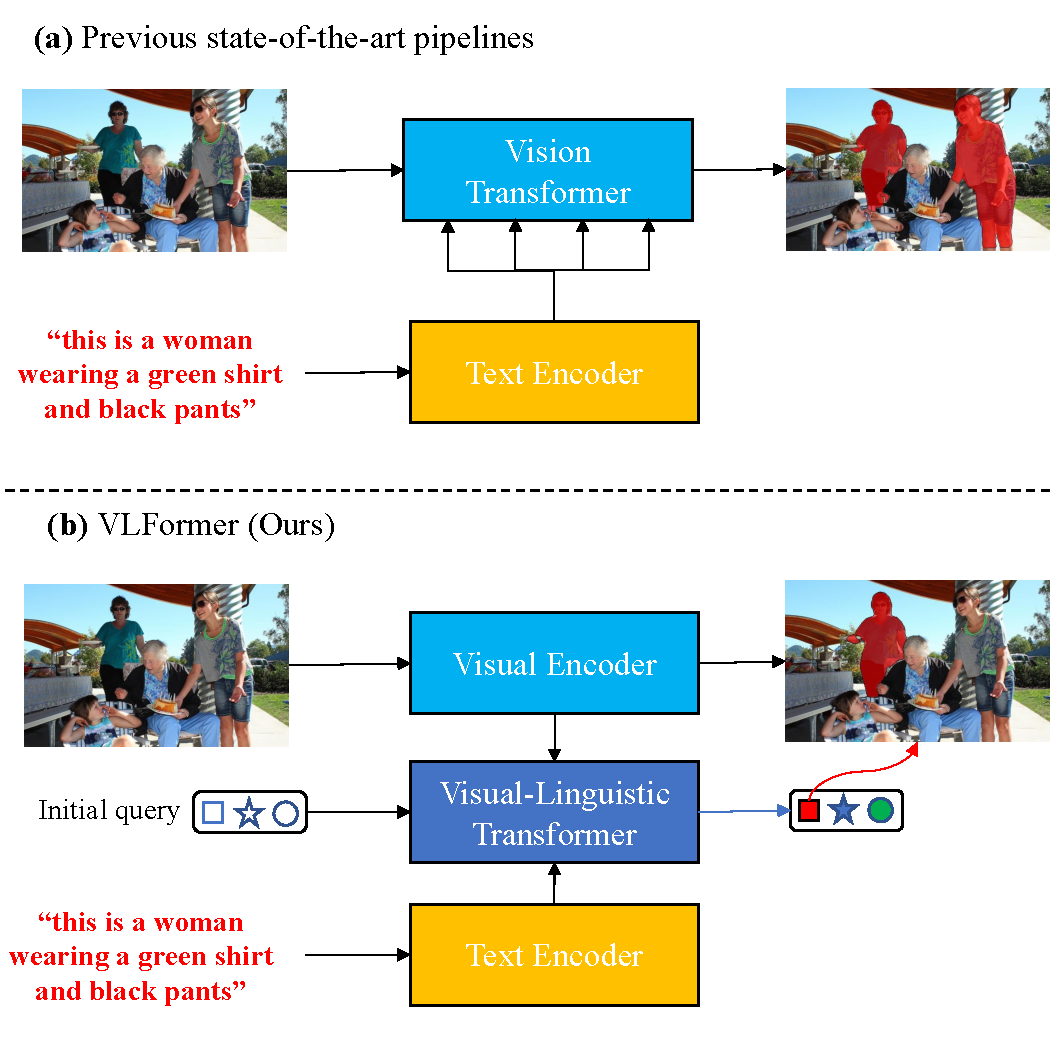
\includegraphics[width=0.7\linewidth]{content/resources/images/referring_segmentation/CompareOverview.pdf}
    \caption{Comparison of referring image segmentation pipelines. (a) The previous state-of-the-art approach (i.e., LAVT \cite{yang_lavt_2022}) integrate linguistic features into visual features of a vision transformer model to benefit the jointly exploiting vision-language cues. (b) We propose to leverage a Transformer-based module to associate both visual and linguistic information with a set of object queries, aiming to gradually update the representation of these object queries. The final object queries then produce the mask prediction.}
    \label{fig:comparison_pipeline}
\end{figure}

\vspace{-2mm}
In most previous transformer-based works in computer vision \cite{carion_end--end_2020, wang_end--end_2021, cheng_per-pixel_2021, cheng_masked-attention_2022}, a set of queries is used to represent the class or instance features for detection and segmentation. In referring segmentation task, some works \cite{ding_vision-language_2021, wu_language_2022} generate the query vectors from language features using vision-guided attention or directly. Then these queries are updated in a Transformer decoder using visual features only. It can lead to a problem that the linguistic information can vanish in the object query features after several Transformer decoder layers. To address this issue, a potential solution is to exploit a multi-modal Transformer for simultaneously aggregating visual and linguistic features during the transformer decoder.

Besides, on such referring segmentation problems, the text query usually contains information about the category, position on the image, and appearance of the object. In some cases, the related position between the referred object and others is mentioned. CLIP \cite{radford_learning_2021} models are learned from a wide range of visual concepts followed by the natural language. Hence, these models can better capture the information related to the visual concepts. 


Hence, we propose a Visual-Linguistic Transformers (VLFormer) \citeown{nguyen_vlformer_2022} approach to leverage a set of queries that understand both visual and linguistic features to represent potential objects. First, the CLIP Text Encoder is utilized for linguistic features from natural language expression. The linguistic features are used to improve the vision-language fusion and enhance the representation of object queries through the Transformer-based module. Second, a Visual-Linguistic Transformer, which contains several Visual-Linguistic Transformer Block modules, is designed for constructing fine-grained object features using linguistic and multi-scale visual information. Each Visual-Linguistic Transformer Block (VLB) utilizes the cross-attention modules from linguistic and visual features to object queries, then generates more informative object queries. Figure~\ref{fig:comparison_pipeline} highlights the difference between our proposed work and the state-of-the-art method.
\section{Motivation}
\label{section:motivation}

This is motivation.
\section{Objectives}
\label{sec:objectives}

Our main objective is to apply artificial intelligence to the search system to make it \textbf{smarter} (i.e., more flexible queries, more functionalities) and at the same time \textbf{explainable}, while maintaining \textbf{scalability} (i.e., can operate with a large quantity of data).

This is much broader than just building an AI model as we are building a system that consists of many components. For example, using a top-performing yet slow model may forbid the system to run in real-time. A bad user interface might prevent the user from getting any value out of our system at all. Therefore, to achieve our multiple goals, we have to think about the system's architecture and the interaction between various components. Specifically, we look for simple yet effective solutions as they are easier to scale and also simpler to reason about.

With this in mind, our proposed work has the following main contributions:

\begin{itemize}
    \item \textbf{Scalable architecture}: we separate our application into modules to enhance the maintainability and scalability of the whole system. Specifically, we propose the adoption of a \textbf{vector database} to store the embeddings generated by AI models for use in searching, besides using an ordinary database for storing metadata. This approach prevents the AI model from becoming the bottleneck of the system, enabling querying speed comparable to non-AI systems.
    \item \textbf{Practical guidelines}: we compile our extensive experience from varying users to form a list of guidelines, or principles, for users to keep in mind while searching. This gives users some sense of direction while still being flexible enough to adapt to different situations. Our experience is based on a time-pressured setting dealing with difficult queries, so it should be practical enough.
    \item \textbf{Attention on Explainability}: we enhance our system with a novel \textbf{referring expression segmentation} module to precisely point out the object or concept referred to in the image. This strengthens the model's credibility in all scenarios, especially in some critical ones such as medical uses.
\end{itemize}

\vspace{-2mm}
Our system design is further analyzed in Section \ref{chap-first}, the best practices are listed in Section \ref{sec:best_practices}, and lastly our referring expression segmentation sub-system is described in detail in Section \ref{chap-refer-seg}.
 
%  This inspire us to build a \textbf{scalable} system that can handle a large quantity of data while being relatively simple. Moreover, we try to systematize \textbf{best search practices} from our experience as a kind of "user manual" to help guide the user. Finally, we integrate a \textbf{referring expression object segmentation} module to visualize the objects and concepts being mentioned, providing explainability for our system.
\section{Project content}
% \section{Thesis content}
\label{sec:thesis_content}

After \textbf{Chapter 1}, the remainder of our project is composed of four chapters as follows:

% After \textbf{Chapter 1}, the remainder of our thesis is composed of four chapters as follows:

\textbf{Chapter 2: Related Works}

In this chapter, we first introduce an overview of the main approaches for the Interactive Retrieval System and previous versions of our system.
We then discuss several methods used in Referring Expression Segmentation tasks. Finally, we discuss state-of-the-art approaches in Semi-supervised Video Object Segmentation that we leverage as a post-process to further boost our performance.

\textbf{Chapter 3: Flexible Interactive Retrieval System}

In this chapter, we go into detail about our retrieval system called \textbf{FIRST}. First, we outline the overview of our retrieval system. Following sections describe the design of our system and AI-related components in retrieval process. Finally, we provide more details about the Lifelog Search Challenge 2022 and Visual Browser Showdown 2022, the evaluation metrics used in these challenges, and the result of our interactive retrieval system on each challenge.

\textbf{Chapter 4: Referring Expression Segmentation}

In this chapter, we present our Referring Expression Segmentation framework \textbf{VLFormer} in detail. We first introduce an overview of our framework. Next, we describe each part of our architecture and how efficiently we train the network. Then, an extension to video data is provided. Finally, we discuss about challenges we participated in, the datasets we conducted the experiments, and analyze our performance in both quantitative and qualitative aspects. 

\textbf{Chapter 5: Conclusion}

In this chapter, we summarize our work and briefly discuss the potential improvements of the current approach for future research.

